\section{Árboles generales}
Los Tipos Abstractos de Datos arborescentes se utilizan para representar datos organizados en jerarquías, como podría ser un árbol genealógicoo una estructura de directorios y archivos de un sistema operativo.\newline

Entonces, es importante comprender cómo se constituye un árbol. Para ello, veamos algunos conceptos básicos.

\begin{defi}[Nodo]\label{def nodo}
	Un \textit{nodo} es un punto de intersección, conexión o unón de varios elementos. En el caso que nos ocupa, será un registro que contendrá un dato de interés y, al menos, un puntero para referenciar a otro nodo.
\end{defi}

\begin{obs}
	Un solo nodo forma un árbol $a$. Se dirá que ese nodo es la \textit{raíz} del árbol. Luego, dados $n$ árboles $a_1, \dots, a_n$, podemos construir un nuevo árbol $a'$ añadiendo un nuevo nodo $r$ como raíz y conectándolo con las raíces de los árboles $a_i, 1 \leq i \leq n$, los cuales se llamarán \textit{subárboles} o \textit{hijos de $a'$}. A $r$ se le llamará \textit{padre} de las raíces de estos subárboles.
\end{obs}

% Inicio gráfica árboles


\tikzset{every picture/.style={line width=0.75pt}} %set default line width to 0.75pt        
\begin{center}
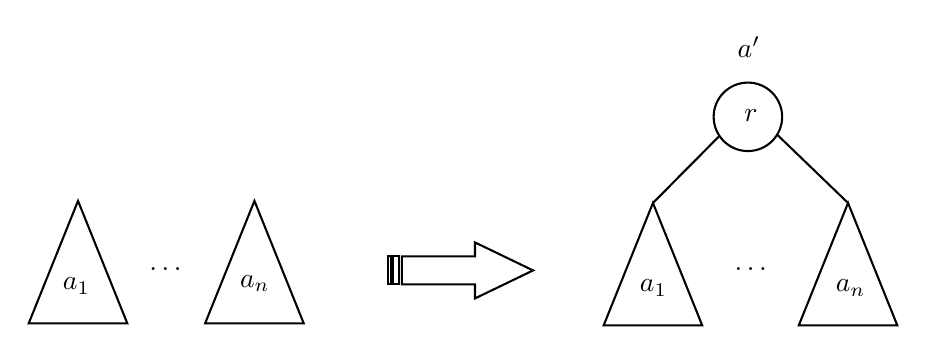
\begin{tikzpicture}[x=0.75pt,y=0.75pt,yscale=-1,xscale=1]
%uncomment if require: \path (0,204); %set diagram left start at 0, and has height of 204

%Shape: Triangle [id:dp10996608333087465] 
\draw   (155.75,121) -- (179.5,180) -- (132,180) -- cycle ;
%Shape: Triangle [id:dp790264761603528] 
\draw   (240.75,121) -- (264.5,180) -- (217,180) -- cycle ;
%Striped Right Arrow [id:dp4866233788869734] 
\draw   (311.75,147.75) -- (347,147.75) -- (347,141) -- (375,154.5) -- (347,168) -- (347,161.25) -- (311.75,161.25) -- cycle ;\draw   (305,147.75) -- (306.35,147.75) -- (306.35,161.25) -- (305,161.25) -- cycle ;\draw   (307.7,147.75) -- (310.4,147.75) -- (310.4,161.25) -- (307.7,161.25) -- cycle ;
%Shape: Circle [id:dp5419639967577192] 
\draw   (462,80.5) .. controls (462,71.39) and (469.39,64) .. (478.5,64) .. controls (487.61,64) and (495,71.39) .. (495,80.5) .. controls (495,89.61) and (487.61,97) .. (478.5,97) .. controls (469.39,97) and (462,89.61) .. (462,80.5) -- cycle ;
%Shape: Triangle [id:dp8770015608859049] 
\draw   (432.75,122) -- (456.5,181) -- (409,181) -- cycle ;
%Shape: Triangle [id:dp9850851144344236] 
\draw   (526.75,122) -- (550.5,181) -- (503,181) -- cycle ;
%Straight Lines [id:da3319007242869292] 
\draw    (432.75,122) -- (464.5,90) ;


%Straight Lines [id:da8442549298704125] 
\draw    (526.75,122) -- (492.5,89) ;



% Text Node
\draw (155,162) node  [align=left] {$a_1$};
% Text Node
\draw (241,161) node  [align=left] {$a_n$};
% Text Node
\draw (433,163) node  [align=left] {$a_1$};
% Text Node
\draw (528,163) node  [align=left] {$a_n$};
% Text Node
\draw (480,80) node  [align=left] {$r$};
% Text Node
\draw (479,47) node  [align=left] {$a'$};
% Text Node
\draw (199,154) node  [align=left] {\dots};
% Text Node
\draw (481,154) node  [align=left] {\dots};


\end{tikzpicture}
\end{center}
% Fin gráfica árboles

\begin{defi}[Hojas]\label{def hojas}
	Se llaman \textit{hojas}  a los nodos del árbol que no tienen hijos. Al resto de nodos se les llamará \textit{nodos internos}.
\end{defi}

\begin{defi}[Nodos hermanos]\label{def nodos hermanos}
	 Dos nodos que comparten padre se dice que son \textit{hermanos}.
\end{defi}

\begin{defi}[Camino]\label{def camino}
	Un \textit{camino} es una sucesión de nodos en la que cada nodo es padre del siguiente. Al número de nodos en un camino se le llama \textit{longitud}.
\end{defi}

\begin{defi}[Rama]\label{def rama}
	Una \textit{rama} es cualquier camino que empieza en la raíz y acaba en una hoja.
\end{defi}

\begin{defi}[Nivel]\label{def nivel}
	El \textit{nivel} o \textit{profundidad} de un nodo es la longitud del camino que va desde la raíz hasta él. En particular, el nivel de la raíz es el $1$.
\end{defi}

\begin{defi}[Altura]\label{def altura}
	La \textit{altura} o \textit{talla} de un árbol es el máximo de los niveles de todos los nodos del árbol.
\end{defi}

\begin{defi}[Grado]\label{def grafo}
	El \textit{grado} o \textit{aridad} de un nodo es su número de hijos.
\end{defi}

\begin{defi}[Antepasado/Descendiente]\label{def antepasado}
	Decimos que un nodo $\alpha$ es \textit{antepasado} de $\beta$ (respectivamente, $\beta$ es \textit{descendiente} de $\alpha$) si existe un camino desde $\alpha$ hasta $\beta$.
\end{defi}

Distinguimos distintos tipos de árboles en función de sus características:
\begin{itemize}
	\item \underline{Árboles ordenados o no ordenados:} un árbol es \textit{ordenado} si el orden de los hijos de cada nodo es relevante. No debe confundirse este tipo de árbol ordenado, basado en la estructura de árbol, con los árboles binarios de búsqueda, en los que el orden está basado en el valor de los nodos del árbol.
	\item \underline{Árboles $n$--arios:} un árbol es \textit{ $n$--ario} si el máximo número de hijos de cualquier nodo es $n$. Los \textit{árboles generales} son la unión de todos los $n$--arios.
	\item \underline{Árboles binarios:} un \textit{árbol binario} es un árbol ordenado cuyos nodos siempre tienen dos hijos (el izquierdo y el derecho), aunque estos pueden ser vacíos.
\end{itemize}

Como se podrá intuir, existen formas de recorrer esta estructura. Veamos, para un árbol binario, los más importantes:
\begin{itemize}
	\item \underline{Recorrido en profundidad (\textit{DFS}):} 
	\begin{itemize}
		\item Preorden: se visita en primer lugar la raíz del árbol y, a continuación, se recorren en preorden el hijo izquierdo y el hijo derecho.
		\item Inorden: se recorre el hijo izquierdo, después se visita la raíz, y, por último, se recorre el hijo derecho.
		\item Postorden: primero se recorren los hijos izquierdo y derecho (en ese orden), y después se visita la raíz.
	\end{itemize}
	\item \underline{Recorrido en anchura (\textit{BFS}):} intuitivamente, se comienza en la raíz y se exploran todos los vecinos de este nodo. A continuación, para cada uno de los vecinos se exploran sus correspondientes vecinos adyacentes, y así hasta que se recorra todo el árbol.
\end{itemize}

\begin{defi}[Árbol binario de búsqueda]\label{def bin}
	Los \textit{árboles binarios de búsqueda} son árboles binarios cuyos nodos guardan elementos sobre los cuales hay definido un orden total estricto y que satisfacen la siguiente propiedad adicional: el elemento en cada nodo es mayor que todos sus descendientes izquierdos y menor que todos sus descendientes derechos.
\end{defi}

\begin{obs}
	Equivalentemente, o bien el árbol es vacío, o bien el elemento en la raíz es el mayor que los elementos del hijo izquierdo y menor que los elementos del hijo derecho, y recursivamente los dos hijos son a su vez árboles binarios de
	búsqueda.
\end{obs}

\begin{obs}
	Las operaciones de búsqueda, inserción y borrado de un elemento tienen un coste lineal respecto a la altura del árbol. En el caso peor, la altura es lineal respecto al número de nodos; aunque, en promedio, es logarítmica respecto al número de nodos.
\end{obs}

\begin{defi}[Árbol completo]\label{def completo}
	Un árbol de altura $h$ es \textit{completo} cuando todos sus nodos internos tienen el máximo número de hijos no vacíos y todas sus hojas están en el nivel $h$. 
\end{defi}


\begin{center}
\tikzset{every picture/.style={line width=0.75pt}} %set default line width to 0.75pt        

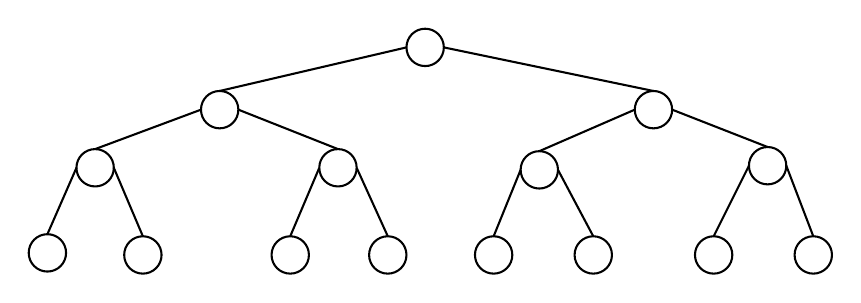
\begin{tikzpicture}[x=0.75pt,y=0.75pt,yscale=-1,xscale=1]
%uncomment if require: \path (0,142); %set diagram left start at 0, and has height of 142

%Shape: Circle [id:dp7019811966058006] 
\draw   (321,21) .. controls (321,16.03) and (325.03,12) .. (330,12) .. controls (334.97,12) and (339,16.03) .. (339,21) .. controls (339,25.97) and (334.97,30) .. (330,30) .. controls (325.03,30) and (321,25.97) .. (321,21) -- cycle ;
%Shape: Circle [id:dp19000564090720107] 
\draw   (402,121) .. controls (402,116.03) and (406.03,112) .. (411,112) .. controls (415.97,112) and (420,116.03) .. (420,121) .. controls (420,125.97) and (415.97,130) .. (411,130) .. controls (406.03,130) and (402,125.97) .. (402,121) -- cycle ;
%Shape: Circle [id:dp776261763000253] 
\draw   (508,121) .. controls (508,116.03) and (512.03,112) .. (517,112) .. controls (521.97,112) and (526,116.03) .. (526,121) .. controls (526,125.97) and (521.97,130) .. (517,130) .. controls (512.03,130) and (508,125.97) .. (508,121) -- cycle ;
%Shape: Circle [id:dp5946274661202907] 
\draw   (460,121) .. controls (460,116.03) and (464.03,112) .. (469,112) .. controls (473.97,112) and (478,116.03) .. (478,121) .. controls (478,125.97) and (473.97,130) .. (469,130) .. controls (464.03,130) and (460,125.97) .. (460,121) -- cycle ;
%Shape: Circle [id:dp424270300255542] 
\draw   (303,121) .. controls (303,116.03) and (307.03,112) .. (312,112) .. controls (316.97,112) and (321,116.03) .. (321,121) .. controls (321,125.97) and (316.97,130) .. (312,130) .. controls (307.03,130) and (303,125.97) .. (303,121) -- cycle ;
%Shape: Circle [id:dp1272803711448881] 
\draw   (256,121) .. controls (256,116.03) and (260.03,112) .. (265,112) .. controls (269.97,112) and (274,116.03) .. (274,121) .. controls (274,125.97) and (269.97,130) .. (265,130) .. controls (260.03,130) and (256,125.97) .. (256,121) -- cycle ;
%Shape: Circle [id:dp7663196163730203] 
\draw   (185,121) .. controls (185,116.03) and (189.03,112) .. (194,112) .. controls (198.97,112) and (203,116.03) .. (203,121) .. controls (203,125.97) and (198.97,130) .. (194,130) .. controls (189.03,130) and (185,125.97) .. (185,121) -- cycle ;
%Shape: Circle [id:dp42227872696040036] 
\draw   (139,120) .. controls (139,115.03) and (143.03,111) .. (148,111) .. controls (152.97,111) and (157,115.03) .. (157,120) .. controls (157,124.97) and (152.97,129) .. (148,129) .. controls (143.03,129) and (139,124.97) .. (139,120) -- cycle ;
%Shape: Circle [id:dp8481496025412734] 
\draw   (486,78) .. controls (486,73.03) and (490.03,69) .. (495,69) .. controls (499.97,69) and (504,73.03) .. (504,78) .. controls (504,82.97) and (499.97,87) .. (495,87) .. controls (490.03,87) and (486,82.97) .. (486,78) -- cycle ;
%Shape: Circle [id:dp9618743637726007] 
\draw   (376,80) .. controls (376,75.03) and (380.03,71) .. (385,71) .. controls (389.97,71) and (394,75.03) .. (394,80) .. controls (394,84.97) and (389.97,89) .. (385,89) .. controls (380.03,89) and (376,84.97) .. (376,80) -- cycle ;
%Shape: Circle [id:dp979262719746538] 
\draw   (431,51) .. controls (431,46.03) and (435.03,42) .. (440,42) .. controls (444.97,42) and (449,46.03) .. (449,51) .. controls (449,55.97) and (444.97,60) .. (440,60) .. controls (435.03,60) and (431,55.97) .. (431,51) -- cycle ;
%Shape: Circle [id:dp46184207652643594] 
\draw   (279,79) .. controls (279,74.03) and (283.03,70) .. (288,70) .. controls (292.97,70) and (297,74.03) .. (297,79) .. controls (297,83.97) and (292.97,88) .. (288,88) .. controls (283.03,88) and (279,83.97) .. (279,79) -- cycle ;
%Shape: Circle [id:dp9945309570418638] 
\draw   (162,79) .. controls (162,74.03) and (166.03,70) .. (171,70) .. controls (175.97,70) and (180,74.03) .. (180,79) .. controls (180,83.97) and (175.97,88) .. (171,88) .. controls (166.03,88) and (162,83.97) .. (162,79) -- cycle ;
%Shape: Circle [id:dp5168033798323237] 
\draw   (222,51) .. controls (222,46.03) and (226.03,42) .. (231,42) .. controls (235.97,42) and (240,46.03) .. (240,51) .. controls (240,55.97) and (235.97,60) .. (231,60) .. controls (226.03,60) and (222,55.97) .. (222,51) -- cycle ;
%Shape: Circle [id:dp5574294830932686] 
\draw   (354,121) .. controls (354,116.03) and (358.03,112) .. (363,112) .. controls (367.97,112) and (372,116.03) .. (372,121) .. controls (372,125.97) and (367.97,130) .. (363,130) .. controls (358.03,130) and (354,125.97) .. (354,121) -- cycle ;
%Straight Lines [id:da0637076717134496] 
\draw    (231,42) -- (321,21) ;


%Straight Lines [id:da7311073015301238] 
\draw    (339,21) -- (440,42) ;


%Straight Lines [id:da38316649426821614] 
\draw    (222,51) -- (171,70) ;


%Straight Lines [id:da5148209876878125] 
\draw    (240,51) -- (288,70) ;


%Straight Lines [id:da461627107071902] 
\draw    (162,79) -- (148,111) ;


%Straight Lines [id:da962981802750262] 
\draw    (180,79) -- (194,112) ;


%Straight Lines [id:da08437473710719923] 
\draw    (297,79) -- (312,112) ;


%Straight Lines [id:da9435716299966027] 
\draw    (279,79) -- (265,112) ;


%Straight Lines [id:da9396459830287123] 
\draw    (394,80) -- (411,112) ;


%Straight Lines [id:da8860486978647262] 
\draw    (376,80) -- (363,112) ;


%Straight Lines [id:da2630671938250324] 
\draw    (431,51) -- (385,71) ;


%Straight Lines [id:da8223605178656174] 
\draw    (449,51) -- (495,69) ;


%Straight Lines [id:da06108809536008308] 
\draw    (486,78) -- (469,112) ;


%Straight Lines [id:da4792026221020784] 
\draw    (504,78) -- (517,112) ;
\end{tikzpicture}
\end{center}

\begin{defi}[Árbol semicompleto]\label{def semicompleto}
	Un árbol de altura $h$ es \textit{semicompleto} si bien es completo o tiene vacantes una serie de posiciones consecutivas del nivel $h$ empezando por la derecha, de tal manera que al rellenar dichas posiciones con nuevas hojas se obtiene un árbol completo.
\end{defi}

\begin{center}
\tikzset{every picture/.style={line width=0.75pt}} %set default line width to 0.75pt        

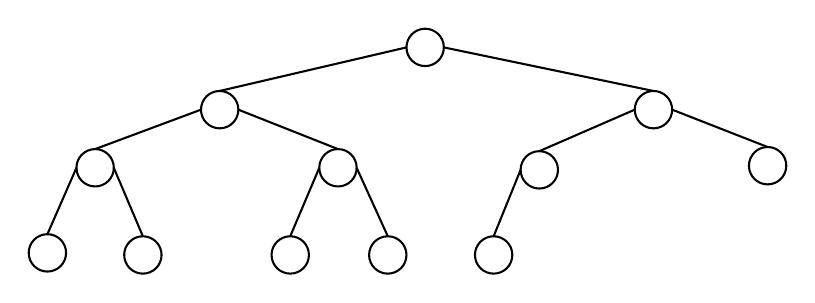
\begin{tikzpicture}[x=0.75pt,y=0.75pt,yscale=-1,xscale=1]
%uncomment if require: \path (0,142); %set diagram left start at 0, and has height of 142

%Shape: Circle [id:dp7019811966058006] 
\draw   (321,21) .. controls (321,16.03) and (325.03,12) .. (330,12) .. controls (334.97,12) and (339,16.03) .. (339,21) .. controls (339,25.97) and (334.97,30) .. (330,30) .. controls (325.03,30) and (321,25.97) .. (321,21) -- cycle ;
%Shape: Circle [id:dp424270300255542] 
\draw   (303,121) .. controls (303,116.03) and (307.03,112) .. (312,112) .. controls (316.97,112) and (321,116.03) .. (321,121) .. controls (321,125.97) and (316.97,130) .. (312,130) .. controls (307.03,130) and (303,125.97) .. (303,121) -- cycle ;
%Shape: Circle [id:dp1272803711448881] 
\draw   (256,121) .. controls (256,116.03) and (260.03,112) .. (265,112) .. controls (269.97,112) and (274,116.03) .. (274,121) .. controls (274,125.97) and (269.97,130) .. (265,130) .. controls (260.03,130) and (256,125.97) .. (256,121) -- cycle ;
%Shape: Circle [id:dp7663196163730203] 
\draw   (185,121) .. controls (185,116.03) and (189.03,112) .. (194,112) .. controls (198.97,112) and (203,116.03) .. (203,121) .. controls (203,125.97) and (198.97,130) .. (194,130) .. controls (189.03,130) and (185,125.97) .. (185,121) -- cycle ;
%Shape: Circle [id:dp42227872696040036] 
\draw   (139,120) .. controls (139,115.03) and (143.03,111) .. (148,111) .. controls (152.97,111) and (157,115.03) .. (157,120) .. controls (157,124.97) and (152.97,129) .. (148,129) .. controls (143.03,129) and (139,124.97) .. (139,120) -- cycle ;
%Shape: Circle [id:dp8481496025412734] 
\draw   (486,78) .. controls (486,73.03) and (490.03,69) .. (495,69) .. controls (499.97,69) and (504,73.03) .. (504,78) .. controls (504,82.97) and (499.97,87) .. (495,87) .. controls (490.03,87) and (486,82.97) .. (486,78) -- cycle ;
%Shape: Circle [id:dp9618743637726007] 
\draw   (376,80) .. controls (376,75.03) and (380.03,71) .. (385,71) .. controls (389.97,71) and (394,75.03) .. (394,80) .. controls (394,84.97) and (389.97,89) .. (385,89) .. controls (380.03,89) and (376,84.97) .. (376,80) -- cycle ;
%Shape: Circle [id:dp979262719746538] 
\draw   (431,51) .. controls (431,46.03) and (435.03,42) .. (440,42) .. controls (444.97,42) and (449,46.03) .. (449,51) .. controls (449,55.97) and (444.97,60) .. (440,60) .. controls (435.03,60) and (431,55.97) .. (431,51) -- cycle ;
%Shape: Circle [id:dp46184207652643594] 
\draw   (279,79) .. controls (279,74.03) and (283.03,70) .. (288,70) .. controls (292.97,70) and (297,74.03) .. (297,79) .. controls (297,83.97) and (292.97,88) .. (288,88) .. controls (283.03,88) and (279,83.97) .. (279,79) -- cycle ;
%Shape: Circle [id:dp9945309570418638] 
\draw   (162,79) .. controls (162,74.03) and (166.03,70) .. (171,70) .. controls (175.97,70) and (180,74.03) .. (180,79) .. controls (180,83.97) and (175.97,88) .. (171,88) .. controls (166.03,88) and (162,83.97) .. (162,79) -- cycle ;
%Shape: Circle [id:dp5168033798323237] 
\draw   (222,51) .. controls (222,46.03) and (226.03,42) .. (231,42) .. controls (235.97,42) and (240,46.03) .. (240,51) .. controls (240,55.97) and (235.97,60) .. (231,60) .. controls (226.03,60) and (222,55.97) .. (222,51) -- cycle ;
%Shape: Circle [id:dp5574294830932686] 
\draw   (354,121) .. controls (354,116.03) and (358.03,112) .. (363,112) .. controls (367.97,112) and (372,116.03) .. (372,121) .. controls (372,125.97) and (367.97,130) .. (363,130) .. controls (358.03,130) and (354,125.97) .. (354,121) -- cycle ;
%Straight Lines [id:da0637076717134496] 
\draw    (231,42) -- (321,21) ;


%Straight Lines [id:da7311073015301238] 
\draw    (339,21) -- (440,42) ;


%Straight Lines [id:da38316649426821614] 
\draw    (222,51) -- (171,70) ;


%Straight Lines [id:da5148209876878125] 
\draw    (240,51) -- (288,70) ;


%Straight Lines [id:da461627107071902] 
\draw    (162,79) -- (148,111) ;


%Straight Lines [id:da962981802750262] 
\draw    (180,79) -- (194,112) ;


%Straight Lines [id:da08437473710719923] 
\draw    (297,79) -- (312,112) ;


%Straight Lines [id:da9435716299966027] 
\draw    (279,79) -- (265,112) ;


%Straight Lines [id:da8860486978647262] 
\draw    (376,80) -- (363,112) ;


%Straight Lines [id:da2630671938250324] 
\draw    (431,51) -- (385,71) ;


%Straight Lines [id:da8223605178656174] 
\draw    (449,51) -- (495,69) ;

\end{tikzpicture}

\end{center}

